\begin{center}
    \vspace*{1.5cm}
    {\fontsize{20}{20}\textbf{\fontspec{Lucida Sans Unicode}Klassiska visor}}\\
    \vspace{0.7cm}
    {\fontsize{12}{12}\textit{Om Bellman själv får välja}}
\end{center}
\addtocwithheader{Klassiska visor}  % Add entry to TOC and set header
\thispagestyle{empty}
\noBackground

\newpage
\resetBackground

\subsection*{Måltidssången} 
\index[alfa]{Måltidssången}
\index[anfa]{Så lunka vi så småning om}
\songinfo{Text: C. M. Bellman \\Fredmans sång N:o 21}

\begin{parse lines}[\noindent]{#1\\}
    Så lunka vi så småningom,
    från Bacchi buller och tumult
    när döden ropar: Granne, kom,
    ditt timglas är nu fullt
    Du gubbe fäll din krycka ner
    och du, du yngling lyd min lag:
    den skönsta nymf som åt dig ler
    inunder armen tag

    Tycker du att graven är för djup,
    nå välan, så tag dig då en sup,
    tag dig sen dito en, dito två, dito tre
    så dör du nöjdare

    Säg, är du nöjd, min granne säg?
    Så prisa värden nu till slut
    om vi har en och samma väg,
    så följoms åt... Drick ut!
    Men först med vinet rött och vitt,
    för vår värdinna bugom oss
    och halkom sen i graven fritt
    vid aftonstjärnans bloss

    Tycker du…
\end{parse lines}

\vissteduatt{Visste du att denna ska sjungas när alla fått sin varmrätt?} %\\ När man sjunger "tycker du..." ska man kroka i arm med sina bordsgrannar    ?\\}

\newpage

% \begin{textblock*}{3cm}(6.0cm,3.0cm)
%     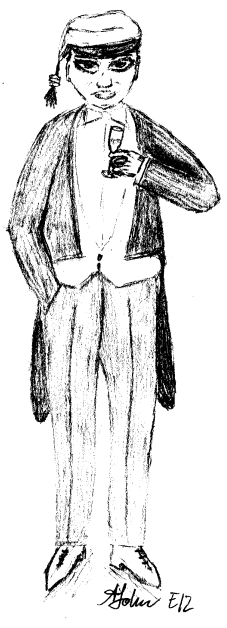
\includegraphics[width=6.5cm, trim=2.5cm 2.5cm 2.1cm 2.2cm, clip]{./bilder/den_blomster_tid_nu_kommer.pdf}
% \end{textblock*}

\begin{textblock*}{2.7cm}(6.5cm,4cm) % {width}(x, y)
    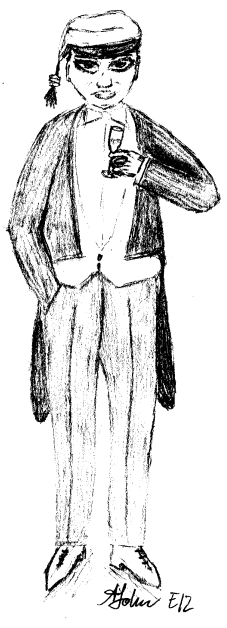
\includegraphics[width=2.8cm]{./bilder/den_blomster_tid_nu_kommer.png}
\end{textblock*}


\subsection*{Den blomstertid nu kommer} 
\index[alfa]{Den blomstertid nu kommer}
\index[anfa]{Den blomstertid nu kommer}
%\songinfo{Svensk sommarpsalm}

\begin{parse lines}[\noindent]{#1\\}
    Den blomstertid nu kommer
    med lust och fägring stor
    Du nalkas, ljuva sommar,
    då gräs och gröda gror
    Med blid och livlig värma
    till allt som varit dött,
    sig solens strålar närma,
    och allt blir återfött

    De fagra blomsterängar
    och åkerns ädla säd,
    de rika örtesängar
    och lundens gröna träd,
    de skola oss påminna
    Guds godhets rikedom,
    att vi den nåd besinna
    som räcker året om
\end{parse lines}

\subsection*{Kungssången} 
\index[alfa]{Kungssången}
\index[anfa]{Ur svenska hjärtans djup en gång}
\songinfo{Musik: Otto Lindblad\\Text: C.V.A Strandberg}

%\colorbox{yellow}{OSÄKER PÅ DENNA}
\begin{parse lines}[\noindent]{#1\\}
    Ur svenska hjärtans djup en gång
    en samfälld och en enkel sång,
    som går till kungen fram!
    Var honom trofast och hans ätt,
    gör kronan på hans hjässa lätt,
    och all din tro till honom sätt,
    du folk av frejdad stam! 
\end{parse lines}

\vissteduatt{Visste du att i vissa delar av vårt land inleds alla sittningar \\
med kungssången?}


\newpage
\enlargethispage{1cm}
\subsection*{Studentsången} 
\index[alfa]{Studentsången}
\index[anfa]{Sjung om studentens lyckliga dag}
\songinfo{Musik: Prins Gustaf\\
Text: Herman Sätherberg
}

\begin{parse lines}[\noindent]{#1\\}
    ||: Sjung om studentens lyckliga dag,
    låtom oss fröjdas i ungdomens vår!
    Än klappar hjärtat med friska slag,
    och den ljusnande framtid är vår :||

    ||: Inga stormar än
    i våra sinnen bo,
    hoppet är vår vän,
    och vi dess löften tro,
    när vi knyta förbund i den lund,
    där de härliga lagrarna gro!
    där de härliga lagrarna gro! 
    Hurra! :||

\end{parse lines}


\subsection*{Du gamla, du fria} 
\index[alfa]{Du gamla, du fria}
\index[anfa]{Du gamla, du fria}
\songinfo{Text: Richard Dybeck}

\begin{parse lines}[\noindent]{#1\\}
    Du gamla, du fria, du fjällhöga nord
    du tysta, du glädjerika sköna
    Jag hälsar dig vänaste land uppå jord
    ||: Din sol, din himmel, dina ängder gröna :||

    Du tronar på minnen från fornstora dar
    då ärat ditt namn flög över jorden
    Jag vet att du är och du blir vad du var
    ||: Ja, jag vill leva, jag vill dö i Norden :||
\end{parse lines}

% \vissteduatt{visste du att...En händelse som enligt historien bidrog till \\
% att sången började få status som nationalsång var vid en promotionsmiddag \\
% vid Lunds Universitet våren 1893, då Kung Oscar II ställde sig upp när sången framfördes.}

\vissteduattlong{Visste du att enligt historien fick sången status som nationalsång\\
efter en promotionsmiddag vid Lunds universitet 1893, när\\
Kung Oscar II reste sig under framförandet?}

\newpage

\subsection*{O, gamla klang och jubeltid} 
\index[alfa]{O, gamla klang och jubeltid}
\index[anfa]{O, gamla klang och jubeltid}
\songinfo{Mel: O, alte Burschenherrlichkeit!
}

\begin{parse lines}[\noindent]{#1\\}
    O, gamla klang och jubeltid, 
    ditt minne skall förbliva
    och än åt livets bistra strid 
    ett rostigt skimmer giva!
    Snart tystnar allt vårt yra skämt,
    vår sång blir stum, vårt glam förstämt;
    o jerum, jerum, jerum,
    o, quae mutatio rerum!

    Var äro de, som kunde allt,
    blott ej sin ära svika,
    som voro män av äkta halt
    och världens herrar lika?
    De drogo bort från vin och sång
    till vardagslivets tråk och tvång;
    o, jerum, jerum, jerum,
    o, quae mutatio rerum!

    En tämjer forsens vilda fall,
    en annan ger oss papper,
    en idkar maskinistens kall,
    en mästrar volt så tapper,
    en ritar hus, en mäter mark,
    en blandar hop mixtur så stark;
    o, jerum, jerum, jerum,
    o, quae mutatio rerum!
\end{parse lines}

\vissteduatt{Visste du att denna sång sjungs när en sittning ska avlutas på \\flera andra sektioner?}

\newpage

\begin{parse lines}[\noindent]{#1\\}
    Men hjärtat i en sann student
    kan ingen tid förfrysa,
    den glädjeeld, som där han har tänt,
    hans hela liv skall lysa.
    Det gamla skalet brustit har,
    men kärnan finnes frisk dock kvar,
    och vad han än må mista,
    den skall dock aldrig brista!

    Så sluten, bröder, fast vår krets
    till glädjens värn och ära!
    Trots allt vi tryggt och väl tillfreds
    vår vänskap trohet svära.
    Lyft bägarn högt, och klinga, vän!
    De gamla gudar leva än
    bland skålar och pokaler,
    bland skålar och pokaler!
\end{parse lines}

\vissteduatt{Visste du att den tredje versen är LTH:s och KTH:s egna vers?}

\newpage

\subsection*{Längtan till landet} 
\index[alfa]{Längtan till landet}
\index[anfa]{Vintern rasat ut bland våra fjällar}
\songinfo{Musik: O. Lindblad\\ Text: H. Sätherberg}

\begin{parse lines}[\noindent]{#1\\}
    Vintern rasat ut bland våra fjällar,
    drivans blommor smälta ned och dö
    Himlen ler i vårens ljusa kvällar
    solen kysser liv i skog och sjö
    ||: Snart är sommar'n här! I purpurvågor,
    guldbelagda, azurskiftande
    ligga ägnarne i dagens lågor
    och i lunden dansa källorne :||

    Ja, jag kommer! Hälsen glada vindar
    ut till landet, ut till fåglarne,
    att jag älskar dem, till björk och lindar,
    sjö och berg, jag vill dem återse
    ||: Se dem än som i min bardoms stunder
    följa bäckens dans till klarnad sjö
    Trastens sång i furuskogens lunder,
    vattenfågelns lek kring fjärd och ö :||
\end{parse lines}

\vissteduatt{Visste du att sången sjungs av Lunds studentsångare 1:a maj varje\\år för att fira in våren?}

\newpage

\subsection*{Nu grönskar det} 
\index[alfa]{Nu grönskar det}
\index[anfa]{Nu grönskar det i dalens famn}
\songinfo{Mel: "Bondekantaten" (BWV 212) av J. S. Bach\\
Text: Evelyn Lindström}

\begin{parse lines}[\noindent]{#1\\}
    Nu grönskar det i dalens famn,
    nu doftar äng och lid
    Kom med, kom med på vandringsfärd
    i vårens glada tid!
    Var dag är som en gyllne skål,
    till brädden fylld med vin
    Så drick, min vän, drick sol och doft,
    ty dagen den är din

    Långt bort från stadens gråa hus
    vi glatt vår kosa styr,
    och följer vägens vita band
    mot ljusa äventyr
    Med öppna ögon låt oss se
    på livets rikedom
    som gror och sjuder överallt
    där våren går i blom!
\end{parse lines}

\newpage


\subsection*{Brevet från kolonien} 
\index[alfa]{Brevet från kolonien}
\index[anfa]{Hejsan morsan, hejsan stabben}
\songinfo{Cornelis Vreeswijk}

%\colorbox{yellow}{OSÄKER PÅ DENNA}

\begin{parse lines}[\noindent]{#1\\}
    Hejsan morsan, hejsan stabben
    Här är brev från älsklingsgrabben
    Vi har kul på kolonien
    Vi bor tjugoåtta gangstergrabbar i en

    Stor barack med massa sängar
    Kan ni skicka mera pengar?
    För det vore en god gärning
    Jag har spelat bort vartenda dugg på tärning

    Här är roligt vill jag lova
    Fastän lite svårt att sova
    Killen som har sängen över mig
    Han vaknar inte han när han behöver, nej

    Jag har tappat två framtänder
    För jag skulle gå på händer
    När vi lattjade charader
    Så när morsan nu får se mig får hon spader

    Ute i skogen finns baciller
    Men min kompis han har piller
    Som han köpt utav en ful typ
    Och om man äter dem blir man en jättekul typ
\end{parse lines}

\newpage

\begin{parse lines}[\noindent]{#1\\}
    Våran fröken är försvunnen
    Hon har dränkt sig uti brunnen
    För en morgon blev hon galen
    När vi släppte ut en huggorm i matsalen

    Men jag är inte, rädd för spöken
    För min kompis han har kröken
    Som han gjort utav potatis
    Och som han säljer i baracken nästan gratis

    Föreståndaren han har farit
    Han blir aldrig var han varit
    För polisen kom och tog hand
    Om honom förra veckan när vi lekte skogsbrand

    Ute i skogen finns det rådjur
    I baracken finns det smådjur
    Och min bäste kompis Tage
    Han har en liten fickkniv inuti sin mage

    Honom ska de operera
    Ja, nu vet jag inge mera
    Kram och kyss och hjärtligt tack sen
    Men nu ska vi ut och bränna grannbaracken
\end{parse lines}

\newpage
